%%%%%%%%%%%%%%%%
% Ceci est un exemple de modèle de CV créé en utilisant altacv.cls
% (v1.3, 10 mai 2020) écrit par LianTze Lim (liantze@gmail.com). Compile maintenant avec pdfLaTeX, XeLaTeX et LuaLaTeX.
%
%% Il peut être distribué et/ou modifié sous les
%% conditions de la licence publique LaTeX Project, soit version 1.3
%% de cette licence ou (à votre discrétion) toute version ultérieure.
%% La dernière version de cette licence se trouve dans
%%    http://www.latex-project.org/lppl.txt
%% et la version 1.3 ou ultérieure fait partie de toutes les distributions de LaTeX
%% version 2003/12/01 ou ultérieure.
%%%%%%%%%%%%%%%%

%% Si vous utilisez \orcid ou les icônes academicons
%% assurez-vous d'avoir l'option academicons
%% ici, et compilez avec XeLaTeX
%% ou LuaLaTeX.
% \documentclass[10pt,a4paper,academicons]{altacv}

%% Utilisez l'option "normalphoto" si vous voulez une photo normale au lieu d'un recadrage circulaire
% \documentclass[10pt,a4paper,normalphoto]{altacv}

\documentclass[10pt,a4paper,ragged2e,withhyper]{altacv}

%% AltaCV utilise les polices fontawesome5 et academicons
%% et packages.
%% Voir http://texdoc.net/pkg/fontawesome5 et http://texdoc.net/pkg/academicons pour la liste complète des symboles. Vous DEVEZ compiler avec XeLaTeX ou LuaLaTeX si vous voulez utiliser academicons.

% Modifiez la mise en page si nécessaire
\geometry{left=1.1cm,right=1cm,top=1.5cm,bottom=1.5cm,columnsep=1.2cm}

% Le package paracol permet de composer des colonnes de texte en parallèle
\usepackage{paracol}

% Changez la police si vous le souhaitez, selon que
% vous utilisez pdflatex ou xelatex/lualatex
\ifxetexorluatex
  % Si vous utilisez xelatex ou lualatex:
  \setmainfont{Roboto Slab}
  \setsansfont{Lato}
  \renewcommand{\familydefault}{\sfdefault}
\else
  % Si vous utilisez pdflatex:
  \usepackage[rm]{roboto}
  \usepackage[defaultsans]{lato}
  \usepackage{graphicx}
  % \usepackage{sourcesanspro}
  \renewcommand{\familydefault}{\sfdefault}
\fi

% Modifiez les couleurs si vous le souhaitez
\definecolor{VividPurple}{HTML}{3E0097}
\definecolor{SlateGrey}{HTML}{2E2E2E}
\definecolor{LightGrey}{HTML}{666666}
\colorlet{name}{black}
\colorlet{tagline}{VividPurple}
\colorlet{heading}{VividPurple}
\colorlet{headingrule}{VividPurple}
\colorlet{subheading}{VividPurple}
\colorlet{accent}{VividPurple}
\colorlet{emphasis}{SlateGrey}
\colorlet{body}{LightGrey}

% Modifiez certaines polices si nécessaire
\renewcommand{\namefont}{\Huge\rmfamily\bfseries}
\renewcommand{\personalinfofont}{\footnotesize}
\renewcommand{\cvsectionfont}{\LARGE\rmfamily\bfseries}
\renewcommand{\cvsubsectionfont}{\large\bfseries}

% Modifiez les puces pour itemize et le marqueur d'évaluation
% pour \cvskill si vous le souhaitez
\renewcommand{\itemmarker}{{\small\textbullet}}
\renewcommand{\ratingmarker}{\faCircle}

%% sample.bib contient vos publications
% \addbibresource{sample.bib}

\begin{document}
\name{Edouard Legoupil}
\tagline{Expert Senior en IA \& Analytique | Automatisation par Système Multi-Agents \& RAG | Data Science | Business Intelligence | Gouvernance des Données}
%% Vous pouvez ajouter plusieurs photos à gauche ou à droite
\photoR{2.8cm}{edouard_pic.jpg}
% \photoL{2.5cm}{Yacht_High,Suitcase_High}

\personalinfo{%
  % Tous ces éléments ne sont pas obligatoires !
  \email{edouard.legoupil@gmail.com}
 % \phone{+34-645-025115}
 % \mailaddress{Adresse, Rue, 00000 Pays}
  %  \location{Valence, Espagne}
 % \homepage{www.homepage.com}
  \twitter{edouard\_lgp}
  \linkedin{edouardlegoupil}
  \github{edouard-legoupil}
  %% Vous DEVEZ ajouter l'option academicons à \documentclass, puis compiler avec LuaLaTeX ou XeLaTeX, si vous voulez utiliser \orcid ou d'autres commandes academicons.
  % \orcid{0000-0000-0000-0000}
  %% Vous pouvez ajouter vos propres détails avec
  %% \printinfo{symbole}{détail}[préfixe de lien hypertexte optionnel]
  % \printinfo{\faPaw}{Hey ho!}[https://example.com/]
  %% Ou vous pouvez déclarer votre propre champ avec
  %% \NewInfoFiled{nomduchamp}{symbole}[préfixe de lien hypertexte optionnel] et l'utiliser :
  % \NewInfoField{gitlab}{\faGitlab}[https://gitlab.com/]
  % \gitlab{votre_id}
}

\makecvheader
%% Selon vos goûts, vous pouvez rendre les polices des environnements itemize légèrement plus petites
% \AtBeginEnvironment{itemize}{\small}

%% Définissez le ratio de largeur des colonnes gauche/droite à 6:4.
\columnratio{0.6}

% Commencez un paracol à 2 colonnes. Les colonnes gauche et droite s'étendront automatiquement
% sur plusieurs pages si le contenu est trop long.
\begin{paracol}{2}


\textbf{Passionné par le potentiel de l'IA à résoudre des défis complexes, je m'épanouis dans des rôles où je peux allier expertise technique et vision stratégique.}

\cvsection{Expérience}

\cvevent{Chief Data Officer, Département ICT}{OIM, Organisation Internationale pour les Migrations}{Juillet 2024 -- En cours}{Valence, Espagne}
\begin{itemize}

\item  Feuille de route IA & Machine Learning : Développement de stratégies pour déployer des solutions d'IA, notamment pour les RH et la gestion de projets.

\item  Gouvernance des données : Mise en place de cadres de gouvernance pour assurer la conformité et la sécurité des données.

\item  Optimisation des plateformes : Audit du \href{https://github.com/iom/powerBI_audit}{compte Power BI Premium}, promotion d'outils d'analyse en libre-service.

\item Management : Constitution et formation d'une équipe décentralisée d'expert données.

\item Innovation : Développement de \href{https://github.com/orgs/iom/repositories?q=language%3AR}{packages R} pour rationaliser les pipelines de données et la génération de rapport.


\end{itemize}

\divider

\cvevent{Évaluateur Régional Principal, Bureau Régional pour les Amériques}{HCR, Haut Commissariat des Nations Unies pour les Réfugiés}{Jan 2024 -- Juin 2024}{Ciudad del Saber, Panama}
\begin{itemize}
\item Définition \& gestion des évaluations de stratégies nationales (Honduras, Péru, Brésil), Supervision des consultants et mission de terrain
\item Prototypage d'un \href{https://edouard-legoupil.github.io/rag_extraction/}{système d'IA/RAG} pour réinjecter les résultats des Evaluations dans les Plans Stratégiques Pluriannuels.
\end{itemize}

\divider

\cvevent{Analyste de Données Régional Principal, Bureau Régional pour les Amériques}{HCR, Haut Commissariat des Nations Unies pour les Réfugiés}{Jan 2020 -- Déc 2023}{Ciudad del Saber, Panama}
\begin{itemize}
\item  \href{https://unhcrverse.github.io/unhcrverse/learn/}{Développement d'outil et formation d'analyste} d'enquêtes auprès des ménages à haute fréquence.  
\item Étalonnage et création \href{https://rstudio.unhcr.org/SeverityIndex/}{d'outils de développement (Shiny)} d'indicateur composite de vulnérabilité.
\end{itemize}

\divider

\cvevent{Responsable de la Gestion de l'Information, Déploiement d'Urgence pour l'Ouragan Dorian}{ Global Cluster Protection, Nations Unies}{Sept 2019 -- Déc 2019}{Nassau \& Marsh Harbour, Bahamas}
\begin{itemize}
\item Conseil au Gouvernement pour un système d'enregistrement d'urgence des population affectée.  
\item Évaluation et  \href{https://humanitarian-user-group.github.io/post/compositeindicator/}{l'analyse de la sévérité humanitaire}.  
\end{itemize}

\divider

\cvevent{Responsable Régional Principal de la Gestion de l'Information, Bureau Régional pour le Moyen-Orient et l'Afrique du Nord}{HCR, Haut Commissariat des Nations Unies pour les Réfugiés}{Juin 2015 -- Août 2019}{Amman, Jordanie}
\begin{itemize}
\item Soutien régional sur les évaluations des besoins, le ciblage de l'assistance et l'analyse de situation.  
\item Analyse statistique d'enquêtes ménages échantillonnées et collaboration sur les rapports de la Banque Mondiale.
\end{itemize}

\divider

\cvevent{Responsable de la Gestion de l'Information, Opération en Jordanie}{HCR, Haut Commissariat des Nations Unies pour les Réfugiés}{Juin 2013 -- Mai 2015}{Amman, Jordanie}
\begin{itemize}
\item Analyse de situation et de réponse pour un afflux d'urgence de 600 000 réfugiés syriens.
\item Mise en place d'un système de collecte de données en coordination avec plus de 60 ONG .
\end{itemize}

\divider

\cvevent{Responsable de la Gestion des Données, Centre de Service Global}{HCR, Haut Commissariat des Nations Unies pour les Réfugiés}{Jan 2009 -- Mai 2013}{Budapest, Hongrie}
\begin{itemize}
\item Développement et lancement du premier portail de partage de données du HCR.
\item Gestion d’une base de données géospatiale globale sur les camps de réfugiés.
\end{itemize}

\divider

\cvevent{Responsable SIG Régional, Centre d'Expertise Régional pour l'Afrique de l'Ouest}{HCR, Haut Commissariat des Nations Unies pour les Réfugiés}{Nov 2005 -- Déc 2008}{Accra, Ghana}
\begin{itemize}
\item Conception d’outils de visualisation : Production de cartes statistiques pour optimiser l’allocation des ressources régionales.

\item Support technique et formation du personnel dans les Opérations (Cote d'Ivoire, Mauritanie, Tchad, etc.) 
\end{itemize}
\divider

\cvevent{Chef de Projet : SIG \& Gestion Territoriale}{Gouvernement Local de Guyane Française, Parc Naturel Régional}{Juin 2004 -- Sept 2005}{Cayenne, Guyane Française}

\divider

\cvevent{Gestionnaire de l'Aide Alimentaire (8 000 tonnes de blé)}{Ministère Burundais de l'Agriculture \& Ambassade de France au Burundi}{Juin 2000 -- Déc 2001}{Bujumbura, Burundi}

\divider 

\cvevent{Chercheur sur les Marchés Agricoles}{MADERA - Organisation Non Gouvernementale}{Juin 1999 -- Novembre 1999}{Jalalabad, Afghanistan}

\medskip

\switchcolumn

\cvsection{Devise}
\begin{quote}
``Sans données, vous n'êtes qu'une personne de plus avec une opinion'' \footnotesize W. Edwards Deming 
\end{quote}
\divider
\begin{quote}
``Sans opinion, vous n'êtes qu'une personne de plus avec des données'' \footnotesize Peter Drucker. 
\end{quote}

\cvsection{Reconnu pour}

\cvachievement{\faSlideshare}{Amélioration de la culture data}{Construit une \href{https://unhcr.github.io/koboloadeR/docs/}{base de connaissances}, un \href{https://unhcr.github.io/koboloadeR/docs/}{package} et une \href{https://humanitarian-user-group.github.io/post/first-meeting/}{communauté d'utilisateurs} pour améliorer la capacité à exploiter les données disponibles.}

\divider 

\cvachievement{\faBullseye}{Score de Vulnérabilité pour la Protection}{Conçu une approche conceptuelle innovante et un modèle de mesure pour cibler et articuler l'assistance humanitaire.}

\divider

\cvachievement{\faTrophy}{Prix de l'Innovation du HCR}{Pour le leadership technique dans le développement et le lancement de la \href{http://data.unhcr.org}{Plateforme de Portail de Données Opérationnelles}}

\cvsection{Points forts}

\cvtag{Architecture Data \& Gouvernance}
\cvtag{Agile}
\cvtag{Gestion de projet}
\cvtag{Formateur}

\cvsection{Langues}

\cvskill{Anglais - C2}{6}
\cvskill{Français - C2}{6}
\cvskill{Espagnol - B2}{4}
\cvskill{Langage R-STAT}{6}
\cvskill{Python - LLM/RAG}{4}

\medskip

\cvsection{Compétences}

\cvevent{Support décisionnel}{Conception de collecte de données, Exploration de données, Visualisation de données, Interprétation collaborative et Business Intelligence}{}{} 

\cvevent{Communication}{Présenter des sujets complexes à un public large et diversifié en termes simples avec supports didactiques et visuels efficaces}{}{}

\cvevent{Partage de Connaissance}{Diffusion de méthodes techniques et revue de littérature académique à destination des experts humanitaires}{}{}

\cvsection{Formation}

\cvevent{Mastère en Architecture des SIG et Cartographie}{ENSG, France}{Septembre 2003 -- Juin 2004}{}

\divider

\cvevent{Master en Agro-Économie Internationale et Développement Rural}{ISTOM, France}{Septembre 1998 -- Juin 2001}{}

\divider

\cvevent{DEUG Économie \& Gestion}{Université de Nantes, France}{Septembre 1996 -- Juin 1998}{}

\divider

\cvevent{Classes Préparatoires - Hypokhâgne BL : Philosophie, Sociologie \& Économie}{Lycée Guist'hau, France}{Septembre 1995 -- Juin 1996}{}

%\cvsection{Exposition à la diversité culturelle}

%Professionnelle et personnelle

%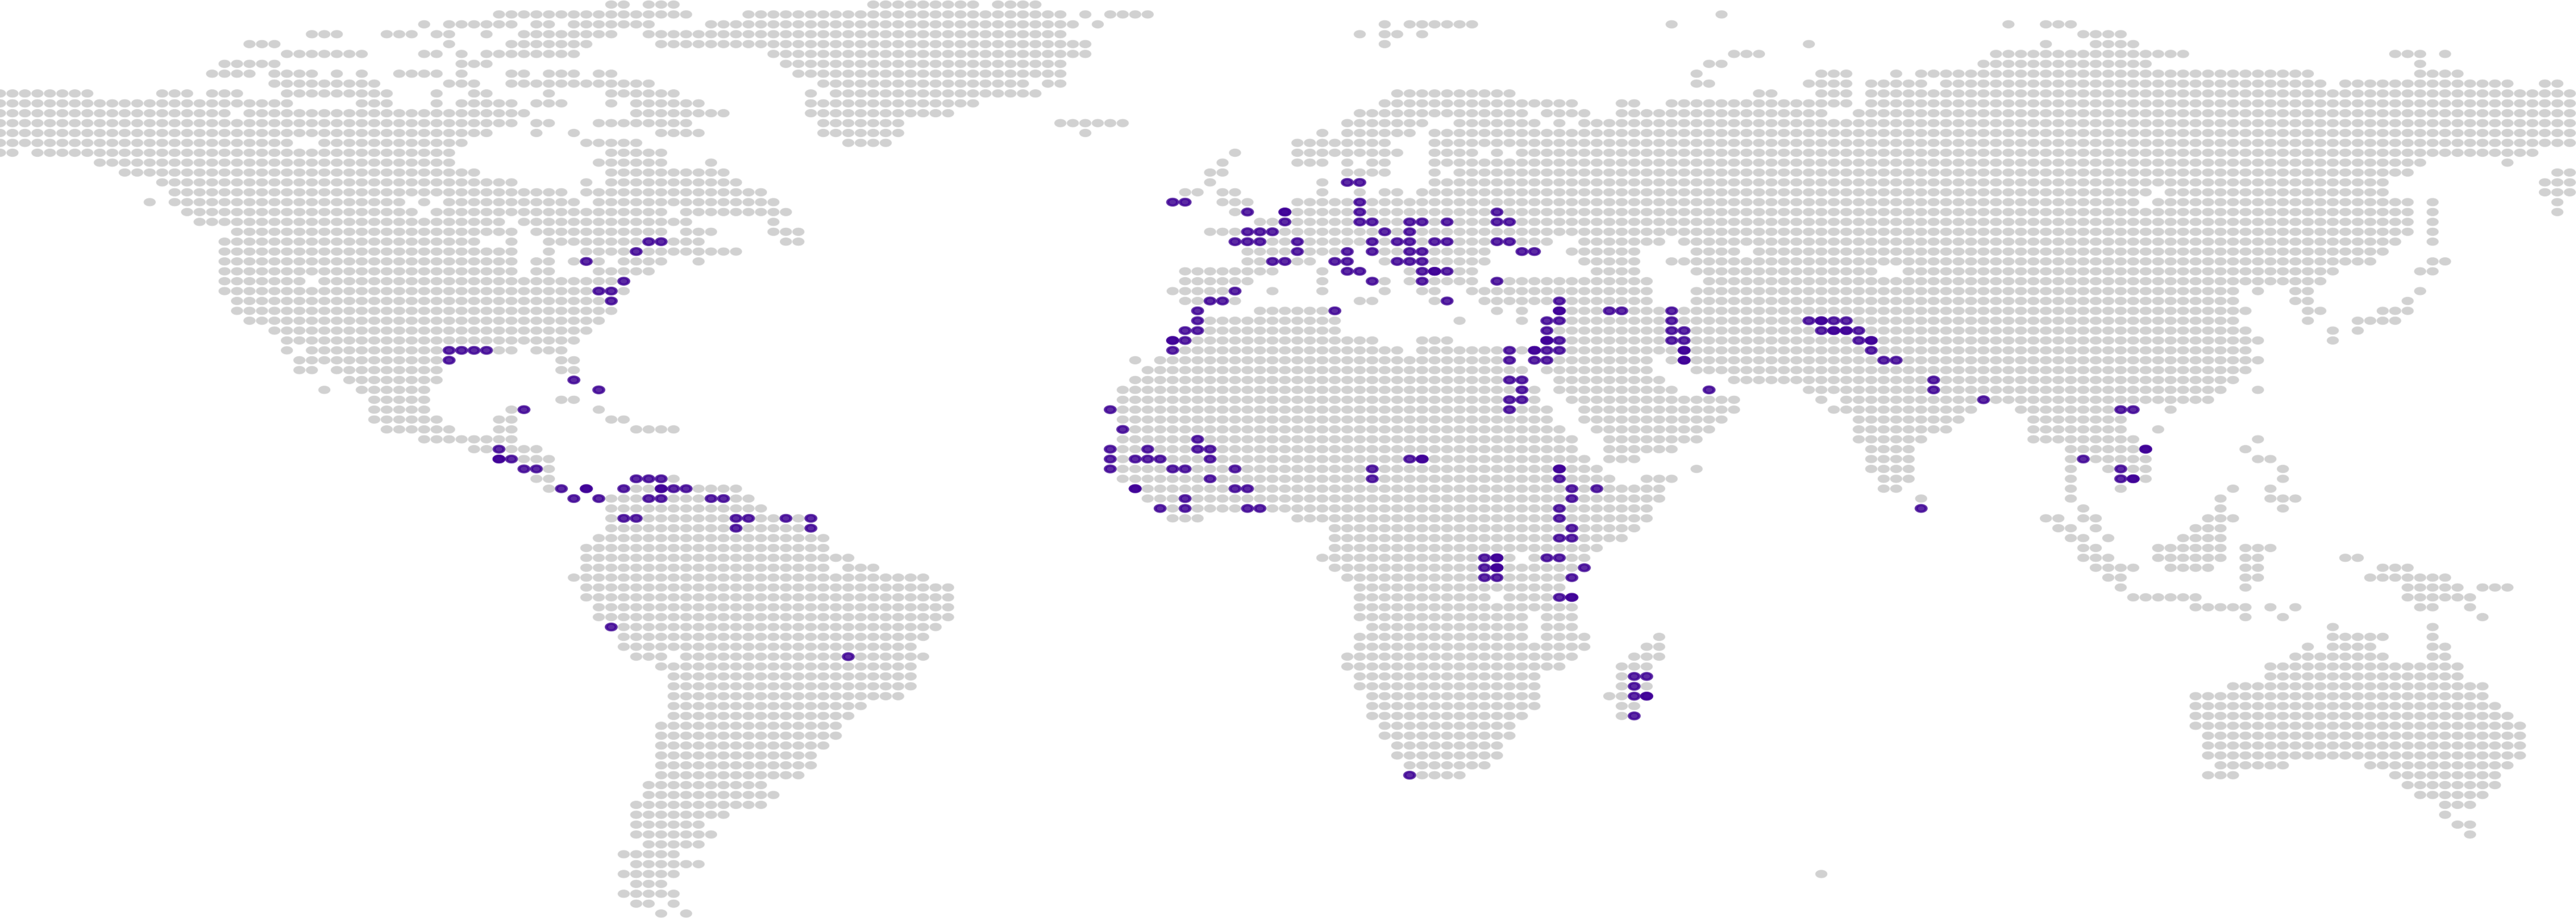
\includegraphics[width=\textwidth]{visited2024_1.png}

\end{paracol}
\end{document}